\NSPage{001}%
\begin{EESegment}{EE-TGT-P001-001}
\begin{center}
  {\Large\bfseries FINITE TIME BLOWUP FOR NAVIER--STOKES\par}
  \vspace{2.5em}
  {\large OPENAI\par}
\end{center}

\vspace{2em}
\noindent\textsc{Abstract.} Viscosity measures how strongly the fluid resists shear. For every
positive viscosity, this paper builds a solution of the three-dimensional incompressible
Navier--Stokes equations. The fluid is incompressible, so
it cannot be squeezed into a smaller volume. It starts at rest. In a finite amount of time its
velocity becomes unbounded, which means that its speed rises past every fixed limit. Its kinetic
energy, the integral of half the squared speed over all space, stays below one fixed finite bound
throughout.
\end{EESegment}

\vspace{3em}
\begin{EESegment}{EE-TGT-P001-002}
\begin{center}
  {\large\textsc{Contents}}
\end{center}
\begin{tabular*}{\textwidth}{@{\extracolsep{\fill}}llr}
1. & Introduction & 1\\
2. & Physical picture of the blowup & 3\\
3. & Outline of the proof & 6\\
4. & Building the leading-order flow & 24\\
5. & Correcting the base flow at every order & 45\\
6. & The auxiliary torus and keeping oscillating supports apart & 62\\
7. & Using oscillations to produce and correct the residual stress & 73\\
8. & Mean corrections with compact support & 88\\
9. & Improving the residual and building the local field & 100\\
10. & Compact forcing and breakdown in the whole space & 116\\
Appendix A. & Matching radial moments and building the heat exterior & 126\\
Appendix B. & Analytic profiles near the axis and continuing them & 144\\
Appendix C. & Producing the admissible stress cone & 157\\
& References & 165
\end{tabular*}
\end{EESegment}

\begin{EESegment}{EE-TGT-P001-003}
\section{Introduction}\label{sec:1}

This paper studies the three-dimensional incompressible Navier--Stokes equations. The main
question is whether a solution that starts from smooth data can develop unbounded velocity in
finite time while its kinetic energy stays bounded. Here smooth means that derivatives of every
order exist and vary continuously. The flow constructed below starts with zero velocity and is
driven by a smooth force with compact support, so the force is zero outside some bounded part of
space and time.
\end{EESegment}

\begin{EESegment}{EE-TGT-P001-004}
\begin{theorem}\label{thm:1.1}
For every \NSi{NS-F-P001-001}{\nu>0}, so for every positive viscosity, there exist a force
\NSi{NS-F-P001-002}{f\in C_c^\infty(\mathbb R^3\times(0,\infty);\mathbb R^3)}, a compact set
\NSi{NS-F-P001-003}{K\subset\mathbb R^3}, and smooth velocity and pressure fields
\NSi{NS-F-P001-004}{u,p} on \NSi{NS-F-P001-005}{\mathbb R^3\times[0,1)} satisfying
\NSFormula{NS-F-P001-006}{display}{1.1}
\begin{equation}
  \partial_tu+(u\cdot\nabla)u-\nu\Delta u+\nabla p=f,
  \qquad \nabla\cdot u=0,
  \qquad u(\cdot,0)=0,
  \tag{1.1}\label{eq:1.1}
\end{equation}
where the notation says that this force is infinitely differentiable, has three components, and
is zero outside a compact part of space and positive time. The condition
\NSi{NS-F-P001-007}{\supp u(\cdot,t)\cup\supp p(\cdot,t)\subset K} holds for every
\NSi{NS-F-P001-008}{0\leq t<1}, which means the velocity and pressure are both zero outside the
same compact set. They also satisfy
\NSFormula{NS-F-P001-009}{display}{none}
\begin{equation*}
  \sup_{0\leq t<1}\lVert u(t)\rVert_{L^2(\mathbb R^3)}<\infty,
  \qquad
  \limsup_{t\uparrow1}\lVert u(t)\rVert_{L^\infty(\mathbb R^3)}=\infty.
\end{equation*}
The first inequality says that the square root of the total squared speed stays below one fixed
bound at every time before one. The second says that, along times approaching one, the largest
speed rises past every fixed bound. So there is no smooth solution
\NSi{NS-F-P001-010}{(u,P)} on
\NSi{NS-F-P001-011}{\mathbb R^3\times[0,\infty)} with the same force and initial
datum whose kinetic energy is uniformly bounded
\NSi{NS-F-P001-012}{\sup_{t\geq0}\frac12\int_{\mathbb R^3}|u(x,t)|^2\,dx<\infty}.
\end{theorem}
\end{EESegment}

\begin{EESegment}{EE-TGT-P001-005}
This proves the option labeled (C) in Fefferman's statement of the Navier--Stokes Millennium
problem \cite{ref-13}. Because the fields have compact support, the same construction also works
on \NSi{NS-F-P001-013}{\mathbb T^3=\mathbb R^3/\mathbb Z^3}, the three-dimensional torus obtained
by identifying points in three-dimensional Euclidean space that differ by an integer vector. This proves option (D)
in \cite{ref-13}; see Corollary~\ref{cor:10.6}.
\end{EESegment}

\NSPage{002}%
\begin{EESegment}{EE-TGT-P002-001}
\subsection{Earlier work and how it leads here}\label{sec:1.1}

The classical Euler equations describe flows that are incompressible and inviscid, meaning that
they have no viscosity \cite{ref-12}.
\NSFormula{NS-F-P002-001}{display}{1.2}
\begin{equation}
  D_tu:=\partial_tu+(u\cdot\nabla)u=-\nabla p+f,
  \qquad \nabla\cdot u=0.
  \tag{1.2}\label{eq:1.2}
\end{equation}
The material acceleration \NSi{NS-F-P002-002}{D_tu} is the acceleration measured while following
one moving parcel, or small moving part, of the fluid. Its velocity changes for two reasons. The flow at a fixed point can change
with time, and the parcel can move to a place where the flow has a different velocity. The term
\NSi{NS-F-P002-003}{(u\cdot\nabla)u} records the second change. It is nonlinear in
\NSi{NS-F-P002-004}{u}, so changing the velocity does not change this term in direct proportion;
this is where most of the difficulty comes from. The first equation is Newton's second law per
unit mass. It says that the parcel's acceleration equals the negative pressure gradient plus the
external force. The second equation says the fluid is incompressible. Squeezing it in one
direction must be matched by stretching it in another.
\end{EESegment}

\begin{EESegment}{EE-TGT-P002-002}
The Navier--Stokes equations \cite{ref-18,ref-21} in \eqref{eq:1.1} add viscosity. The resulting
viscous force resists shear, which is the sliding of neighboring parts of the fluid past one
another. This force is linear in \NSi{NS-F-P002-005}{u}, but it changes the flow in an important
way because it smooths sharp changes in velocity. The regularity problem asks whether that
smoothing always prevents a finite-time singularity in three dimensions. Here a singularity
means that a solution which began smooth stops being smooth after a finite amount of time.
\end{EESegment}

\begin{EESegment}{EE-TGT-P002-003}
In 1934, Leray \cite{ref-16} built global finite-energy weak solutions in three dimensions. They
satisfy an energy inequality, which says that the kinetic energy plus the energy lost through
viscosity is no greater than the starting kinetic energy plus the work done by the force. A weak solution may lack the derivatives
needed to read the equation point by point. Instead, the equation holds after it is integrated
against smooth test fields. Leray's result did not settle whether smooth starting data always give a solution
that stays smooth. Caffarelli, Kohn, and Nirenberg \cite{ref-5} studied suitable weak solutions,
which satisfy an energy inequality not just for the flow as a whole, but also after a smooth cutoff
limits the calculation to part of space and time. They proved that the set
of space-time points where such a solution may be singular has zero one-dimensional parabolic
Hausdorff measure. In this measurement, a space ball of a given radius is paired with a time
interval whose length scales like that radius squared. Zero one-dimensional parabolic Hausdorff
measure means that, no matter how small a positive total length is requested, the singular set can
be covered by such space-time cylinders whose spatial radii add up to less than that length. This
still allows isolated singularities. Escauriaza, Seregin, and Šverák
\cite{ref-11} proved regularity for the unforced Cauchy problem, meaning the initial-value problem
with no external force, when the scale-invariant
\NSi{NS-F-P002-006}{L_t^\infty L_x^3} norm is bounded. This norm first measures the velocity in
space with exponent three and then takes its largest essential value over time, so changing the value on a set of
times of measure zero does not change the norm. Scale-invariant means that the standard change
of space, time, and velocity that leaves the Navier--Stokes equations unchanged also leaves this
norm unchanged.
\end{EESegment}

\begin{EESegment}{EE-TGT-P002-004}
Tao \cite{ref-22} proved finite-time blowup for an averaged version of Navier--Stokes whose
nonlinear term still cancels out of the kinetic-energy balance, as it does in the original
equations. For the original equations,
Buckmaster and Vicol \cite{ref-4} used convex integration, a method that builds a solution by
adding finer and finer oscillating corrections. They obtained nonuniqueness among finite-energy
weak solutions, so the same data can lead to more than one such solution. Albritton, Brué, and
Colombo \cite{ref-1} later built two distinct suitable Leray--Hopf solutions with zero starting
velocity and the same force. A Leray--Hopf solution is a global finite-energy weak solution that
obeys the energy inequality. Their construction uses an unstable vortex written in similarity
variables, which rescale space and time around the possible singularity. Their force belongs to
\NSi{NS-F-P002-007}{L_t^1L_x^2}, so its spatial size with exponent two is integrable in time, but the force
is singular at the initial time.
\end{EESegment}

\begin{EESegment}{EE-TGT-P002-005}
Lifschitz and Hameiri, and Friedlander and Vishik \cite{ref-17,ref-14}, developed methods that
follow a wavevector and a velocity polarization along a background flow. The wavevector records
the direction and spatial frequency of the oscillation, while the polarization records the
direction in which its velocity moves. Craik and Criminale \cite{ref-9} built exact waves of
finite amplitude on affine background flows, whose velocity depends linearly on position up to
a constant term. Their waves work because the quadratic interaction of each wave with itself
cancels. Other earlier results include the centrifugal-instability criteria of Leibovich and
Stewartson \cite{ref-15} and of Billant and Gallaire \cite{ref-2,ref-3}, which test when a rotating
flow is unstable, and the exact viscous shearing waves of Singh and Sridhar \cite{ref-19}.
Daneri and Székelyhidi \cite{ref-10} used oscillations in Euler flows to produce a prescribed
stress, so the required momentum-flux field is chosen first and the oscillations are built to
match it.
\end{EESegment}

\begin{EESegment}{EE-TGT-P002-006}
Córdoba and Martínez-Zoroa \cite{ref-6} built finite-time singularities for the forced
three-dimensional Euler equations. Their construction repeatedly amplifies vortex layers while
concentrating each new layer more tightly. Córdoba, Martínez-Zoroa, and Zheng \cite{ref-8}
extended the method to hypodissipative Navier--Stokes, where the viscous term uses a smaller
positive power of the Laplacian than the usual equation does. Their force lies in a local well-posedness class,
which is regular enough to give short-time existence and uniqueness. These papers developed a
way to form a singularity by passing amplification from one scale to the next while keeping the
external force regular. Strain, the stretching and squeezing caused by the flow, acts on a larger
scale and amplifies vorticity, the local spinning motion, on a smaller scale. The construction
keeps each smaller layer's main interaction with itself from entering the leading equations, and
also keeps that layer from feeding back onto the larger scales. For the incompressible porous-media equation, a different model for flow through a
porous material, Córdoba and Martínez-Zoroa \cite{ref-7} built singularities from smooth starting
data by repeatedly amplifying oscillating layers. Each higher-order approximation cancels more
of the error. As a result, every spatial derivative of the source has one fixed bound that works
at every time. The construction in this paper also uses dynamical amplification,
\end{EESegment}

\NSPage{003}%
\begin{EESegment}{EE-TGT-P003-001}
where the motion of the flow itself makes small disturbances grow. Here those growing
disturbances do a different job. Oscillating pulses produce a mean momentum flux, the average
transport of momentum through the fluid, and that transport provides the force missing from a
background vortex as it collapses.
\end{EESegment}

\begin{EESegment}{EE-TGT-P003-002}
\section{How the blowup happens}\label{sec:2}

First, this section describes what the flow in Theorem~\ref{thm:1.1} is doing. Section~\ref{sec:3}
then gives a full sketch of the proof, showing its main steps before the later sections give all
the details.
\end{EESegment}

\begin{EESegment}{EE-TGT-P003-003}
For any incompressible flow \NSi{NS-F-P003-001}{u} and pressure
\NSi{NS-F-P003-002}{p}, the external force \NSi{NS-F-P003-003}{f} can always be set equal to the
residual in \eqref{eq:1.1}, the result of adding up the four terms on its left-hand side. The
Navier--Stokes equations then hold by construction, because the force was chosen to equal that
result. The hard part is choosing a flow that blows up while this residual stays smooth.
Even though any one of the four terms in the momentum residual may become unbounded, the terms
must cancel one another so that their sum and all its derivatives still extend smoothly through
the singular time, when the velocity becomes unbounded.
\end{EESegment}

\begin{EESegment}{EE-TGT-P003-004}
The construction uses a vortex whose leading profile is self-similar. This is the profile kept
before the later corrections are added. As the vortex shrinks, its shape stays the same after
distance and velocity are measured on their new scales. Its radial width, measured away from
the axis, shrinks faster than its axial length, measured along the axis. In the middle of the vortex, fluid
spirals inward while flowing out along the axis. As the core contracts, the speeds around and
along the axis increase, making the sliding between neighboring layers stronger in the
ring-shaped region around the core.
\end{EESegment}

\begin{EESegment}{EE-TGT-P003-005}
Inside the core, the equations for this first profile make its momentum terms balance. Joining
this inner flow to a smooth outer flow whose speed drops with radius
leaves a nonzero residual in the annulus, the ring-shaped region between them. For the
background flow alone, the momentum residual becomes unbounded as
\NSi{NS-F-P003-004}{t\uparrow1}, so it cannot be the smooth force required by the theorem.
Spatially oscillating pulses are added, meaning velocity disturbances that alternate rapidly
across space. Their nonlinear momentum fluxes, the transport of momentum produced by products
of their velocity components, cancel the singular part of this residual. Further corrections
remove the singular errors that remain, leaving a force that extends smoothly through
\NSi{NS-F-P003-005}{t=1}.
\end{EESegment}

\begin{EESegment}{EE-TGT-P003-006}
\subsection{Inside the core}\label{sec:2.1}
The singularity is built to form at the origin at time \NSi{NS-F-P003-006}{t=1}. Cylindrical
coordinates about the vertical axis are used.
\NSFormula{NS-F-P003-007}{display}{none}
\begin{equation*}
  x=(r\cos\theta,r\sin\theta,z),
\end{equation*}
Here \NSi{NS-F-P003-008}{r} is the distance from the axis,
\NSi{NS-F-P003-009}{\theta} is the angle around it, and \NSi{NS-F-P003-010}{z} is height. The
velocity components \NSi{NS-F-P003-011}{u_r}, \NSi{NS-F-P003-012}{u_\theta}, and
\NSi{NS-F-P003-013}{u_z} give the motion toward or away from the axis, around the axis, and
along it. The leading flow \NSi{NS-F-P003-014}{u^{(0)}} is axisymmetric, which means that its
components depend on \NSi{NS-F-P003-015}{r,z,t} but not on
\NSi{NS-F-P003-016}{\theta}.
\end{EESegment}

\begin{EESegment}{EE-TGT-P003-007}
In the middle of the inner region, fluid spirals toward the axis. A dividing layer near
\NSi{NS-F-P003-017}{z=0} separates fluid moving upward from fluid moving downward; see
Figure~\ref{fig:1}. Farther above and below this middle region, the inner profile also contains
flow moving outward from the axis. Pressure drops toward the axis, providing the leading
centripetal force, the inward force that bends the fluid's path around the axis. Its axial
gradient is the rate at which pressure changes with height. Along the axis, this change in pressure
is one of the terms balanced with transport and viscosity. Near the axis, the pressure force in the axial direction points
toward the plane \NSi{NS-F-P003-018}{z=0}.
\end{EESegment}

\begin{EESegment}{EE-TGT-P003-008}
Flow toward the axis helps the vortex spin faster by carrying angular momentum to smaller
radii. The torque on a particle is the rate at which its angular momentum changes. If no torque acts on a
fluid particle, its angular momentum per unit mass \NSi{NS-F-P003-019}{ru_\theta} is conserved,
so it does not change. Moving inward must therefore increase
\NSi{NS-F-P003-020}{u_\theta}. In the actual core, viscosity carries angular momentum outward.
The typical speed still increases because inward transport and loss through viscosity balance
one another. Incompressibility keeps the incoming fluid from piling up near the axis. Flow out
along the axis carries it away, so the inward motion and faster spin can continue.
\end{EESegment}

\begin{EESegment}{EE-TGT-P003-009}
To leading order, the core changes self-similarly. Its velocity profile keeps the same shape
when distances and velocities are measured in their own changing scales. The scales measured
away from and along the axis shrink at different rates.
\end{EESegment}

\NSPage{004}%
\begin{EESegment}{EE-TGT-P004-001}
\begin{figure}[t]
  \centering
  \NSFigurePlaceholder{NS-FIG-1}
  \caption{The middle of the inner core at three successive times
  \NSi{NS-F-P004-001}{t_1<t_2<t_3<1}. Fluid in this region spirals inward. A dividing layer
  near \NSi{NS-F-P004-002}{z=0} separates flow along the axis in one direction from flow in the
  other. As the singular time gets closer, the region where the flow is strongest shrinks and
  its speed rises. Its radius shrinks faster than its height. The drawing exaggerates this
  difference.}\label{fig:1}
\end{figure}%

Write \NSi{NS-F-P004-003}{\tau=1-t} for the time left before the singularity. The two length
scales then obey
\NSFormula{NS-F-P004-004}{display}{none}
\begin{equation*}
  \ell_r\asymp\tau^{1/2},
  \qquad \ell_z\asymp\tau^{1/2-h},
  \qquad 0<h<1/100,
\end{equation*}
The fixed number \NSi{NS-F-P004-005}{h} lies between zero and one hundredth. The statement
marked by \NSi{NS-F-P004-006}{\asymp} means that the ratio of the quantity on its left to the
quantity on its right stays between two fixed positive numbers that do not depend on
\NSi{NS-F-P004-007}{\tau}. Both lengths go to zero, but
\NSi{NS-F-P004-008}{\ell_r/\ell_z\asymp\tau^h\to0}. The core therefore becomes a thinner and
thinner column at the origin. Its volume stays between fixed positive multiples of
\NSi{NS-F-P004-009}{\tau^{3/2-h}}.
\end{EESegment}

\begin{EESegment}{EE-TGT-P004-002}
The typical sizes of the velocities in the leading flow obey
\NSFormula{NS-F-P004-010}{display}{none}
\begin{equation*}
  |u_\theta^{(0)}|,|u_z^{(0)}|\asymp\tau^{-1/2-h},
  \qquad |u_r^{(0)}|=O(\tau^{-1/2}).
\end{equation*}
These are the typical sizes across the core, not the value at every point. In particular, the
velocity around the axis is zero on the axis itself. The upper-bound statement for the radial
velocity means that one fixed constant times the displayed power bounds its size from above when
the time left is small. The flow is smooth at every \NSi{NS-F-P004-011}{t<1}, but its
largest speeds rise past every fixed bound inside a region shrinking toward the origin as
\NSi{NS-F-P004-012}{t\uparrow1}. The core's kinetic energy stays between fixed positive
multiples of \NSi{NS-F-P004-013}{\tau^{1/2-3h}}, so it goes to zero even though the speeds rise.
\end{EESegment}

\begin{EESegment}{EE-TGT-P004-003}
The different velocity scales give different Reynolds numbers. For a typical speed
\NSi{NS-F-P004-014}{U}, distance \NSi{NS-F-P004-015}{\ell}, and viscosity
\NSi{NS-F-P004-016}{\nu}, the Reynolds number \NSi{NS-F-P004-017}{U\ell/\nu} is the viscous
diffusion time \NSi{NS-F-P004-018}{\ell^2/\nu} divided by the travel time
\NSi{NS-F-P004-019}{\ell/U}. It compares how long viscosity takes to spread motion across that
distance with how long the fluid takes to travel the same distance. Using
the core radius as the distance, the angular and radial Reynolds numbers are
\NSFormula{NS-F-P004-020}{display}{none}
\begin{equation*}
  \mathrm{Re}_\theta:=\frac{|u_\theta|\ell_r}{\nu}\asymp\tau^{-h}\longrightarrow\infty,
  \qquad
  \mathrm{Re}_r:=\frac{|u_r|\ell_r}{\nu}=O(1),
\end{equation*}
for each fixed \NSi{NS-F-P004-021}{\nu>0}.
\end{EESegment}

\begin{EESegment}{EE-TGT-P004-004}
The angular Reynolds number grows past every bound, so the fluid makes more and more turns in
the time viscosity takes to spread motion across the core's radius. The radial Reynolds number
stays bounded, so viscosity keeps competing with the inward radial flow.
\end{EESegment}

\NSPage{005}%
\begin{EESegment}{EE-TGT-P005-001}
\begin{figure}[t]
  \centering
  \NSFigurePlaceholder{NS-FIG-2}
  \caption{The shapes of the pulses and the velocities they add. \emph{On the left,} at one fixed
  height, the active part of each pulse fills a complete ring. The close views show the added
  velocities toward or away from the axis and around it. \emph{On the right,} a slice through the
  axis, where each small patch is the cross-section of a complete ring. These close views show
  the added velocities toward or away from the axis and along it. The colors mark the two pulse
  families. This is a schematic of the pulse arrangement, so it does not give the exact active
  positions, spacing, or aspect ratios between width and height.}\label{fig:2}
\end{figure}%

The transport and diffusion rates obey
\NSFormula{NS-F-P005-001}{display}{none}
\begin{equation*}
  \frac{|u_r|}{\ell_r}=O(\tau^{-1}),
  \qquad \frac{|u_z|}{\ell_z}\asymp\tau^{-1},
  \qquad \frac{\nu}{\ell_r^2}\asymp\tau^{-1}.
\end{equation*}
So radial diffusion, transport by the radial flow, and transport by the axial flow all remain in
the leading balance. None of the three becomes too small to affect that balance as the core
contracts. Diffusion along the axis is smaller. Its size
compared with radial diffusion is
\NSFormula{NS-F-P005-002}{display}{none}
\begin{equation*}
  \frac{\nu/\ell_z^2}{\nu/\ell_r^2}
  =\frac{\ell_r^2}{\ell_z^2}
  \asymp\tau^{2h}\longrightarrow0.
\end{equation*}
The ratio goes to zero, so axial diffusion becomes negligible next to radial diffusion on
these scales.
\end{EESegment}

\begin{EESegment}{EE-TGT-P005-002}
The core also has to provide enough shear at its outer edge to make the pulses there grow. Away
from the middle plane, axial flow carries angular momentum from layers that rotate faster. This
helps keep the angular velocity, the rate at which the fluid circles the axis, dropping steeply
as radius increases. With exact reflection symmetry across
\NSi{NS-F-P005-003}{z=0}, the flow above and below the plane would be mirror images, and this
transport would disappear at the middle plane. The same symmetry would force
\NSi{NS-F-P005-004}{u_z(r,0,t)=0}, so there would be no radial shear of the axial velocity, no
change in that velocity with radius, to take its place. The construction instead uses a slightly
asymmetric axial profile, with a small upward bias and nonzero velocity at
\NSi{NS-F-P005-005}{z=0}. The place where rotation gives little amplification is then separate
from the place where the radial shear of the axial velocity vanishes. Near the middle plane,
that radial shear provides the extra amplification. Farther away, rotation already provides
enough.
\end{EESegment}

\begin{EESegment}{EE-TGT-P005-003}
\subsection{The annulus and the pulses}\label{sec:2.2}
At the edge of the core, the inner vortex joins an outer flow across the annulus. The leading
momentum terms balance inside the core, but they no longer balance in this connecting region.
The external force that would keep the background flow going becomes unbounded as
\NSi{NS-F-P005-006}{t\uparrow1}, so it cannot be the smooth external force the construction
needs.
\end{EESegment}

\begin{EESegment}{EE-TGT-P005-004}
The construction adds an oscillating correction, called a perturbation, to the velocity so that
the fluid's own motion supplies the missing momentum transport. The nonlinear advection term,
the part of the equation that records velocity being carried by the flow, lets this perturbation
produce extra momentum fluxes. Because those fluxes change from place to place, they act as an
internal force on the background. This contribution is made to cancel the singular part of the
background residual, leaving only a remainder that extends smoothly through
\NSi{NS-F-P005-007}{t=1}. These internal forces move momentum from one part of the fluid to
another.
\end{EESegment}

\NSPage{006}%
\begin{EESegment}{EE-TGT-P006-001}
The perturbation is a sequence of pulses that oscillate across space. Each pulse is confined to
a small range of radii, heights, and times, but runs all the way around a complete ring. An
exponentially small external force starts each pulse, so its size falls exponentially rather than
as a fixed power when the construction moves to finer scales. The background shear then
makes the pulse grow. Each cylindrical component of the added velocity has average zero around
the ring, but the momentum fluxes made from products of those components need not average to
zero. For example, an outward radial velocity multiplied by a positive surplus in azimuthal
velocity gives a positive outward flux of angular momentum. An inward radial velocity
multiplied by a negative deficit in azimuthal velocity gives the same sign, so it also carries
angular momentum outward. Changing both signs leaves the product unchanged. Axial momentum is
moved in the same way. The total transport into or out of each region is arranged to provide
the contribution missing from the background momentum balance.

\begin{figure}[htbp]
  \centering
  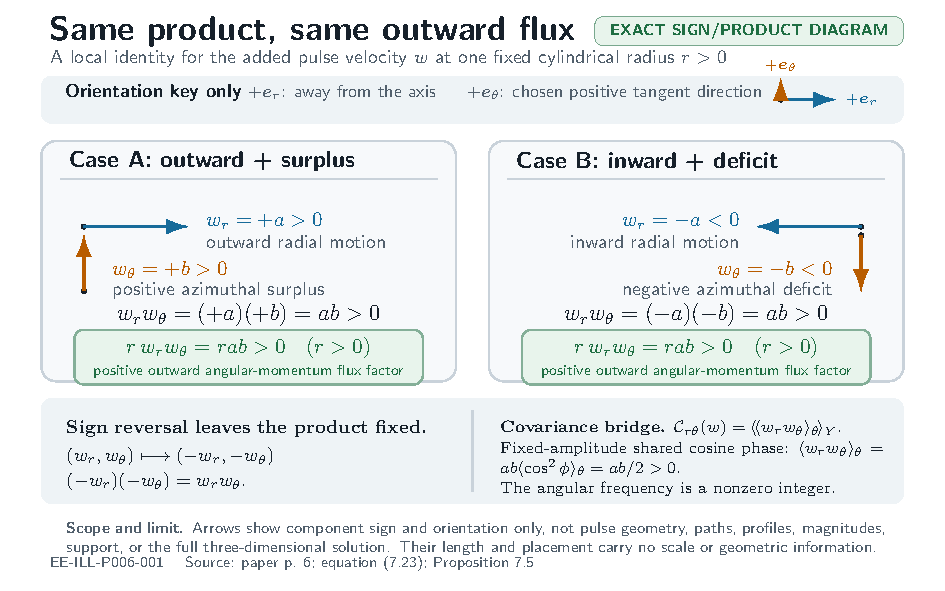
\includegraphics[width=\linewidth]{illustrations/EE-ILL-P006-001-angular-momentum-flux-sign.pdf}
  \caption{Both sign choices give the same positive product. The diagram shows only the signs of
  the radial and azimuthal velocity components at one fixed positive radius. It does not show a
  pulse's shape, path, size, support, or full three-dimensional motion.}
  \label{fig:everyday-flux-sign}
\end{figure}
\end{EESegment}

\begin{EESegment}{EE-TGT-P006-002}
The pulses grow by taking energy from the background shear. A simple rotating flow shows how.
If a patch of fluid moves faster around the axis than the fluid around it, that surplus in
azimuthal velocity produces outward acceleration. If angular velocity drops fast enough as the
radius increases, moving outward makes the patch's surplus larger compared with its new
surroundings. The outward motion and the growing surplus strengthen one another. Together, they
make the pulse grow exponentially whenever the amplification is greater than viscous damping,
the weakening caused by viscosity. In the full flow, shear in the axial velocity also helps the
pulses grow.
\end{EESegment}

\begin{EESegment}{EE-TGT-P006-003}
The same shear also changes the pulse's pattern in space because fluid at different radii
carries that pattern at different speeds. The pulses are pointed in directions that make their
radial wavelength get steadily shorter. As their direction changes, the amplification becomes
weaker. At the same time, the shorter radial wavelength raises the total squared wavenumber,
the squared size of the vector that records the oscillation's spatial frequencies, and this
raises viscous damping. The starting wavelength is chosen so that amplification is larger at
first and damping becomes larger later. The tails of a pulse are the parts near its two time
endpoints, where its size is exponentially small. They are small enough that the errors made by
smoothly switching each pulse on and off, together with every derivative of those errors, vanish
at the singular time.
\end{EESegment}

\begin{EESegment}{EE-TGT-P006-004}
Two pulse families are combined. The families have different ratios of radial angular-momentum
flux to radial axial-momentum flux, so they carry different relative amounts of angular and
axial momentum across radial surfaces. The background profile and the directions of oscillation
are chosen together so that the averaged quadratic velocity products, the averages of products
of two velocity components, provide both components of the required leading stress, the
momentum-flux field needed before the later corrections are added. Pulses appear on finer and
finer spatial and time scales as the
singular time approaches. Further corrections cancel the singular terms still left in the
momentum residual. The resulting velocity becomes unbounded while its residual force extends
smoothly through the singular time.
\end{EESegment}

\begin{EESegment}{EE-TGT-P006-005}
\subsection{The outer flow and the spatial cutoff}\label{sec:2.3}
Outside the annulus, the flow is purely azimuthal and does not change with height. Fluid only
circles the axis there, and its speed drops as the radius increases. Pressure provides the
inward acceleration needed for that circular motion, while viscosity spreads and changes the
azimuthal velocity. This outer flow is chosen to satisfy the radial heat equation exactly, the
diffusion equation with radius as its space variable, so it is called the heat exterior. Its
momentum residual is zero, and no external force is needed to keep this part of the local flow
going.
\end{EESegment}

\begin{EESegment}{EE-TGT-P006-006}
At every fixed radius greater than zero, the outer velocity and pressure approach smooth limits
as the singular time gets closer, and the same is true after any number of derivatives. The
inner construction is also smooth away from the origin. Together these facts make it possible
to cut the flow off smoothly in space, leaving it unchanged near the concentrating core and
making it zero outside a bounded region. The extra force created by this
cutoff stays smooth through the singular time, and the cutoff does not change the concentrating
core.
\end{EESegment}

\begin{EESegment}{EE-TGT-P006-007}
\section{How the proof works}\label{sec:3}

The physical description in Section~\ref{sec:2} leads to an exact cancellation problem. The
velocity and pressure must have a momentum residual that extends smoothly through the singular
time, while the velocity itself becomes unbounded. When viscosity is set equal to one, the
momentum residual is the following expression.
\NSFormula{NS-F-P006-001}{display}{3.1}
\begin{equation}
  \mathscr R(u,p)=\partial_tu+(u\cdot\nabla)u-\Delta u+\nabla p.
  \tag{3.1}\label{eq:3.1}
\end{equation}
\end{EESegment}
